\section{Lecture 11}

Thursday, October 16th 2025. I was gone this day, so I copied notes from J. Liang.

\subsection{Chi-Squared Minimization and Degrees of Freedom}

\begin{itemize}
    \item Degrees of Freedom (dof):
          \[
              \chi^2(\theta) = (y - A \vec{\theta})^T V^{-1} (y - A \vec{\theta})
          \]
    \item At $\hat{\theta}$, $\chi^2$ is minimized:
          \[
              \pdv{\chi^2}{\theta}\bigg|_{\theta = \hat{\theta}} = 0 =
              F(\vec{y} | \vec{\theta}, \vec{x}) =
              \begin{matrix}
                  F(\vec{y} | \theta_1, \vec{x}) \\
                  F(\vec{y} | \theta_2, \vec{x}) \\
                  \vdots                         \\
                  F(\vec{y} | \theta_k, \vec{x})
              \end{matrix}
          \]
    \item i.e. for a linear fit $\vec{y} = A \vec{\theta}$ with $k$ equations:
          \[
              \hat{\theta} = (A^T V^{-1} A)^{-1} (A^T V^{-1}) \vec{y}
          \]
    \item Think about it like this: If I know $n-k$ of the $y_i$'s, the remaining $k$ $y_i$'s are fixed. Their relations might be complex but they are fixed since we have $k$ equations.

          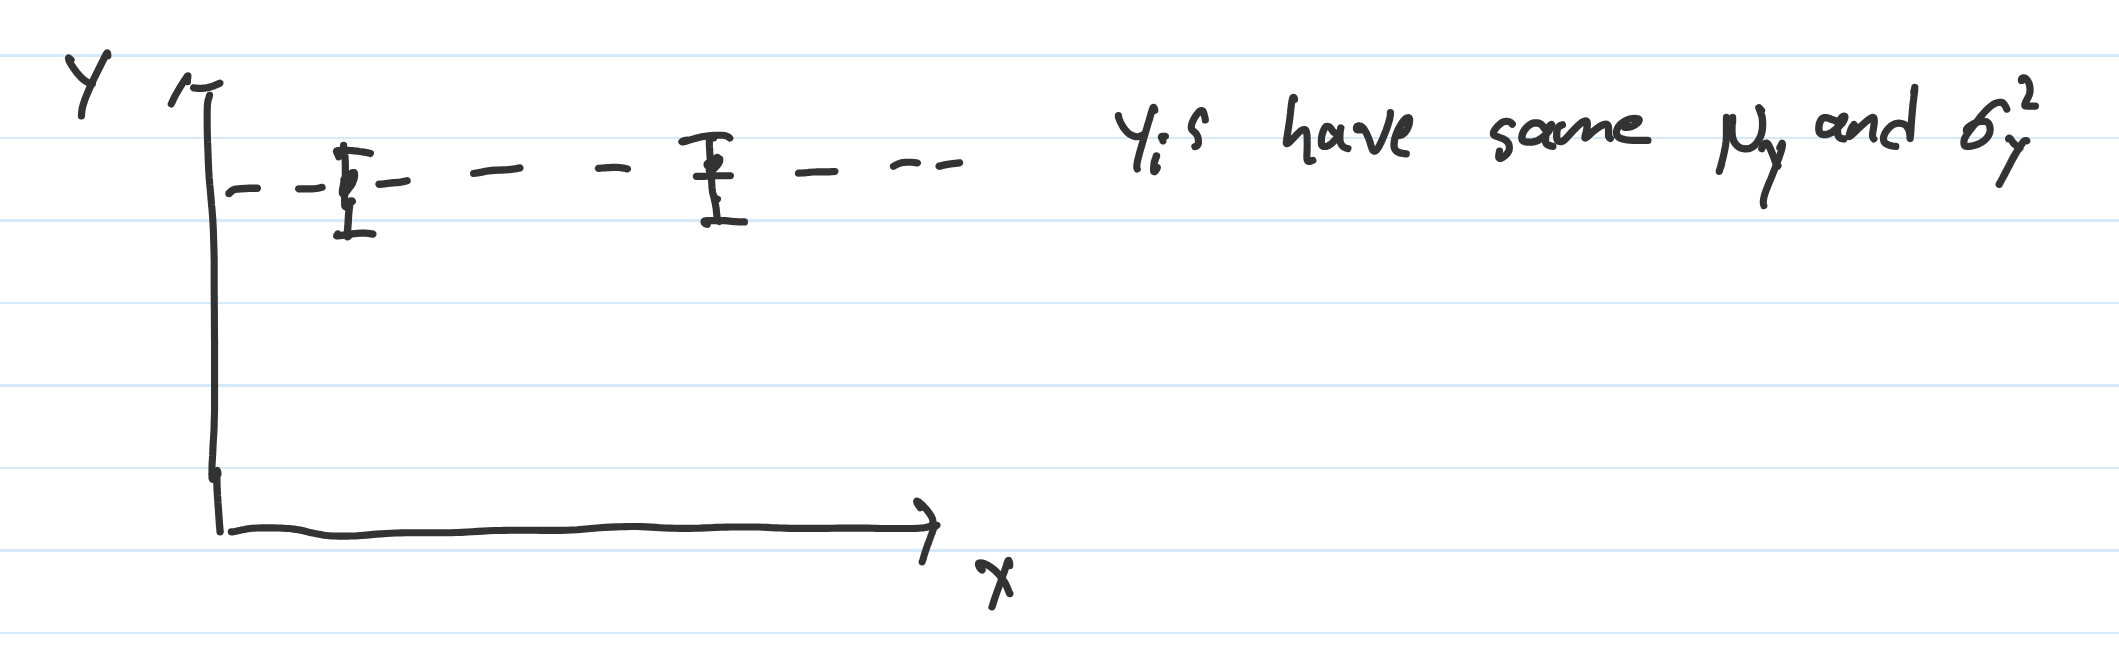
\includegraphics[width=0.8\linewidth]{Images/lec11-chisqu-example.png}

          $y_i$'s have some $N_y$ and $\sigma_y^2$.
\end{itemize}

\subsection{Two-Measurement Example and Correlated Variables}

\begin{itemize}
    \item Best estimator of the true $N$ is $\hat{y} = \frac{y_1 + y_2}{2}$.
          \[
              \chi^2 = \left( \frac{y_1 - \hat{N}}{\sigma_y} \right)^2 +
              \left( \frac{y_2 - \hat{N}}{\sigma_y} \right)^2
          \]
    \item Note:
          \[
              y_1 - \hat{N} = \frac{1}{2} (y_1 - y_2)
          \]
          \[
              y_2 - \hat{N} = \frac{1}{2} (y_2 - y_1)
          \]
    \item Where $z_1 = y_1 - y_2$, and $z_2 = y_2 - y_1$ such that $z_2 = -z_1$.
          \[
              V(z_1, z_2) =
              \begin{pmatrix}
                  1  & -1 \\
                  -1 & 1
              \end{pmatrix}
          \]
    \item Determinant of $V$ is 0, so it is not invertible.
    \item Thus we effectively have only one independent variable.
\end{itemize}

\subsection{Residuals and Goodness of Fit}

\begin{itemize}
    \item Residual: $r_i = y_i - f_i(\vec{\theta})$.
    \item When talking about goodness of fit, people usually divide $\chi^2$ by the number of degrees of freedom (dof). If $\chi^2/\text{dof} \approx 1$, it is a good fit.
    \item What about residuals?

          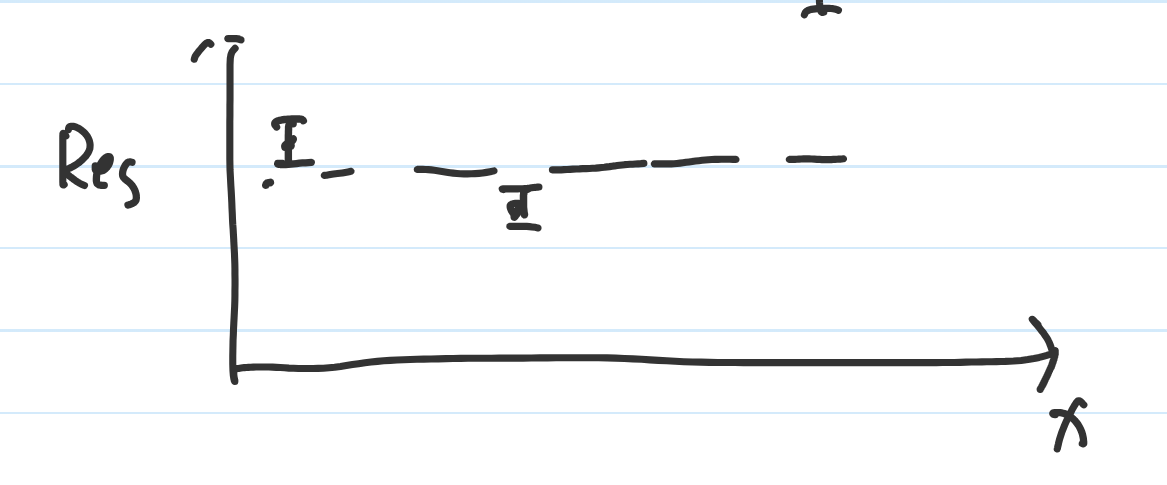
\includegraphics[width=0.5\linewidth]{Images/lec11-residual.png}

          Sometimes one weird data point can throw off the whole $\chi^2$ in unexpected ways, so it is important to check the residuals as well.
    \item If residuals are randomly scattered around 0, it indicates a good fit.
\end{itemize}

\subsection{Distribution of Estimators}

\begin{itemize}
    \item We have been talking about estimators, but we want values of the parameters.
    \item Suppose we perform a fit on a parameter with true value $a$.
    \item From fitting, we get different estimator values from different data sets.

          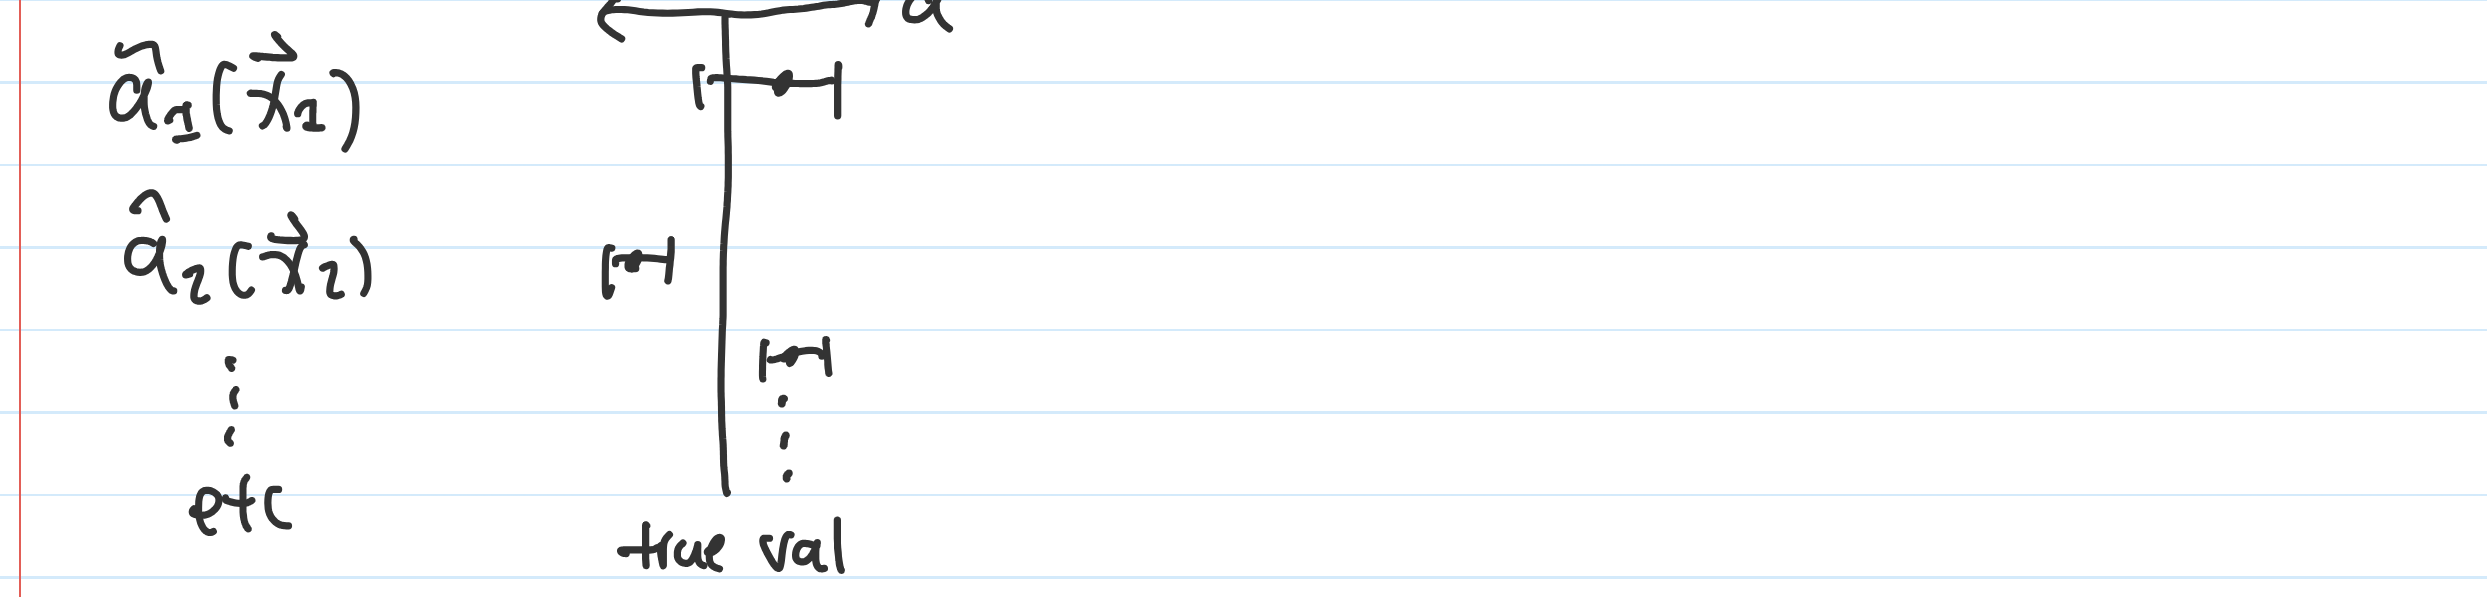
\includegraphics[width=0.5\linewidth]{Images/lec11-spread-est-vals.png}

    \item These estimates can be scattered over a range of values.
\end{itemize}

\subsection{Toy Monte Carlo Simulations for Estimator Distributions}

\begin{itemize}
    \item Toy Monte Carlo:

          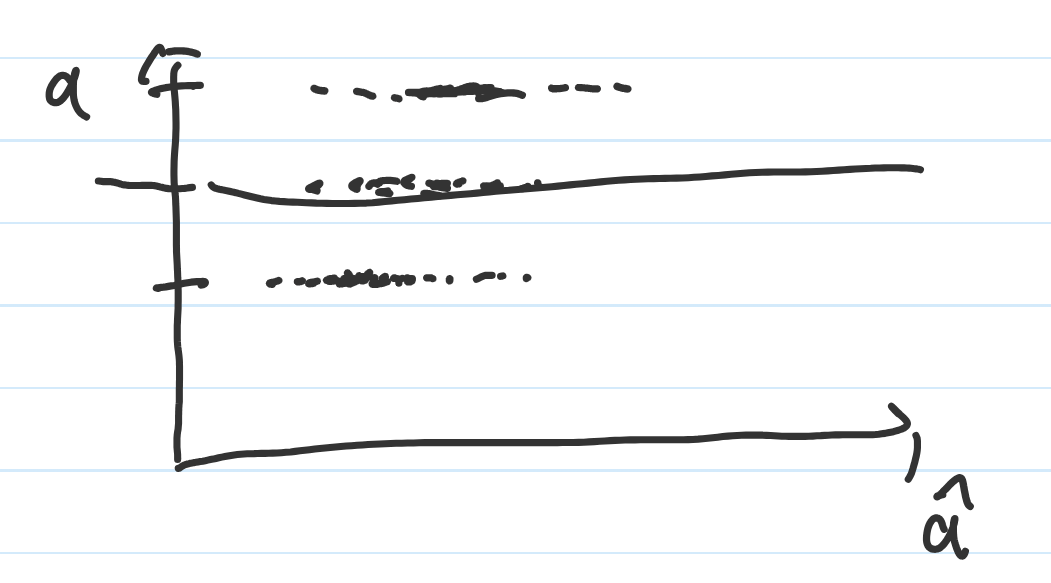
\includegraphics[width=0.6\linewidth]{Images/lec11-toy-monte-carlo.png}

    \item Often, the model is too complicated to get an analytic form of the estimator distribution.
          \begin{enumerate}
              \item Pick a parameter $a$.
              \item Generate many data sets according to the model with parameter $a$.
              \item For each data set, compute the estimator $\hat{a}$.
              \item Plot a histogram of $\hat{a}$.
              \item Repeat steps 2–4 $n$ times.
              \item Repeat step 1 $m$ times.
          \end{enumerate}
    \item For each $a$ value, we can determine e.g. 5\%, 90\%, and 5\% quantiles.

          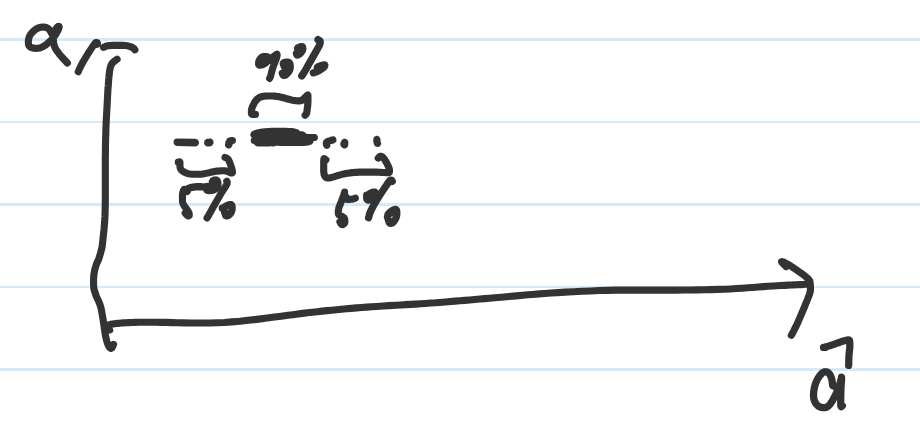
\includegraphics[width=0.6\linewidth]{Images/lec11-mc-intervals.png}

    \item We then connect these points.

          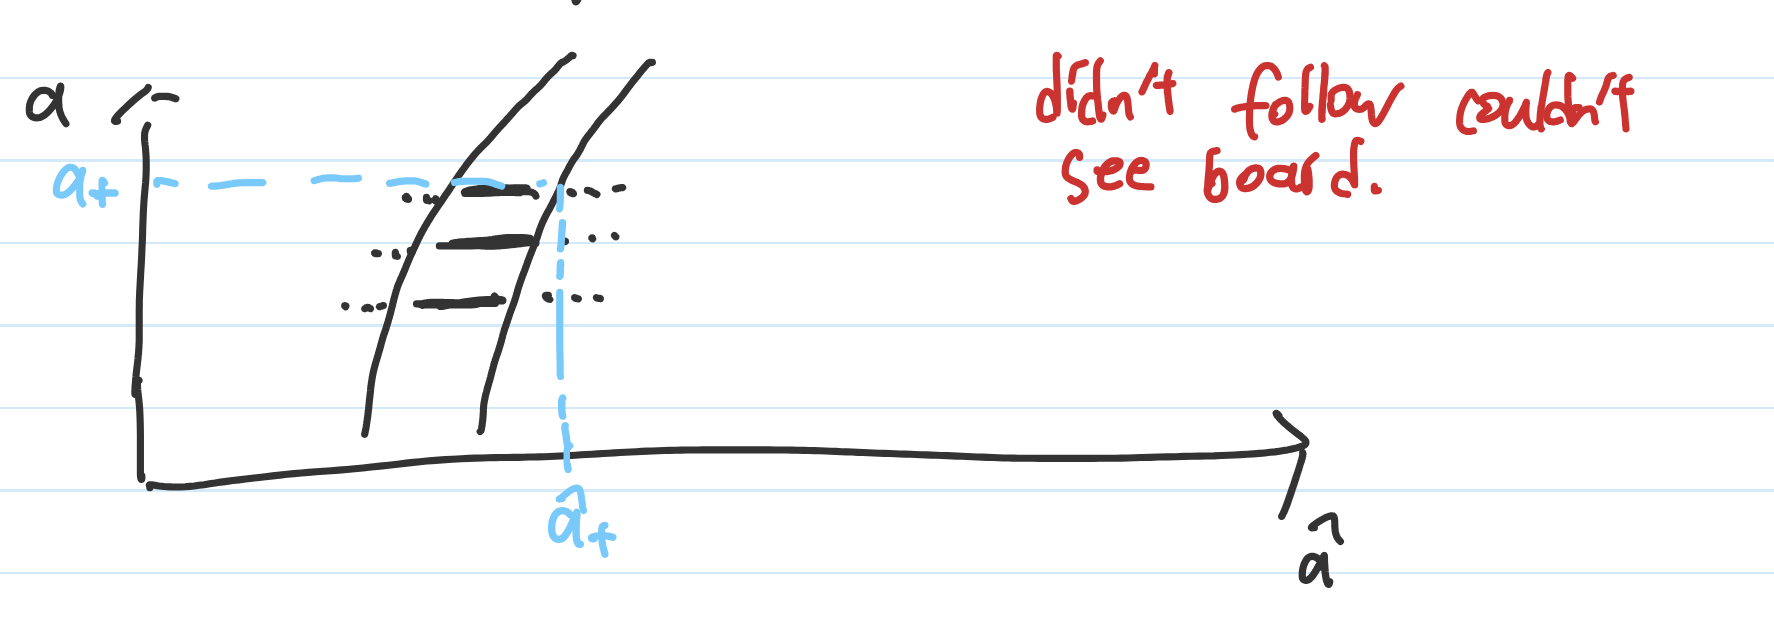
\includegraphics[width=0.6\linewidth]{Images/lec11-fit-connect.png}

    \item $P(a_{-} \leq a \leq a_{+}) = 0.90$.
          Coverage = fraction of time your prescription for the estimator interval contains the true value $a$.
    \item In other words, we find or choose $\hat{a}_{-}$ and $\hat{a}_{+}$ such that 90\% of the time, the true $a$ lies in our interval (corresponding to $a_{-}$ and $a_{+}$).
    \item The bias in all this is that we can really pick intervals however we want.

          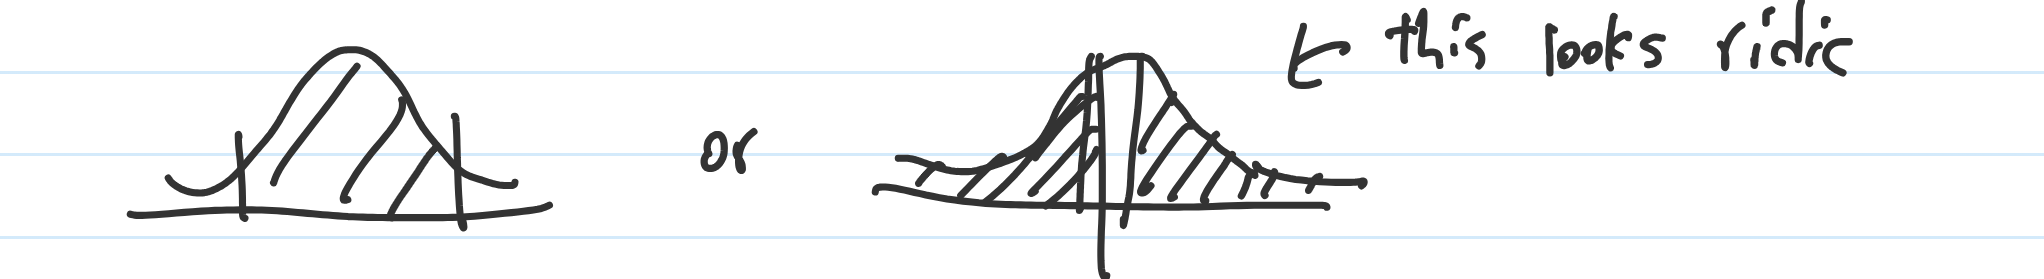
\includegraphics[width=0.6\linewidth]{Images/lec11-biased-intervals.png}
\end{itemize}

\subsection{Typical Applications of Least Squares Fitting}

\begin{itemize}
    \item Typical usage of Least Squares (LS):
          \begin{enumerate}
              \item $x_i$, $y_i$, with known $\sigma_x$, and known $\sigma_y$ for $y_i$.

                    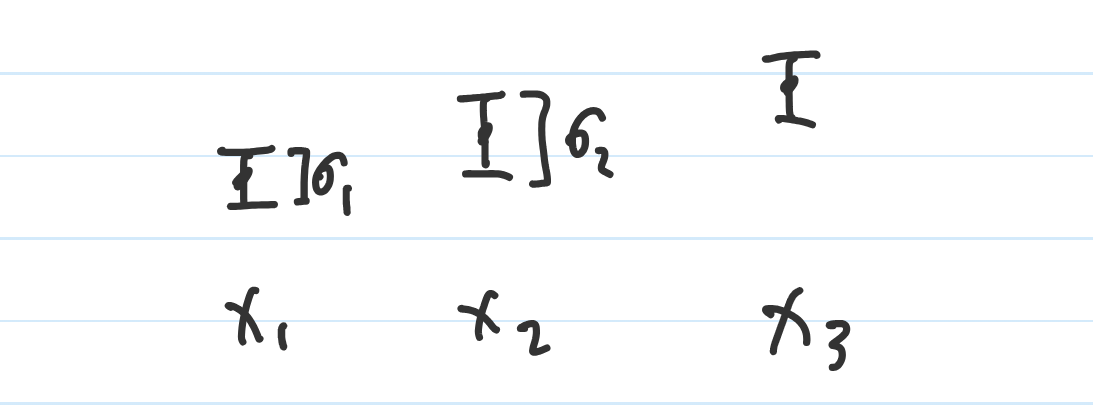
\includegraphics[width=0.4\linewidth]{Images/lec11-points.png}

                    If $y_i$'s are measured by a detector, we can determine $\sigma_i$ by analyzing the detector.
              \item Histograms: i.e., measure $x$ on a coordinate, which can have resolution effects, etc., where $y =$ statistics of the number of events at the same $x$.

                    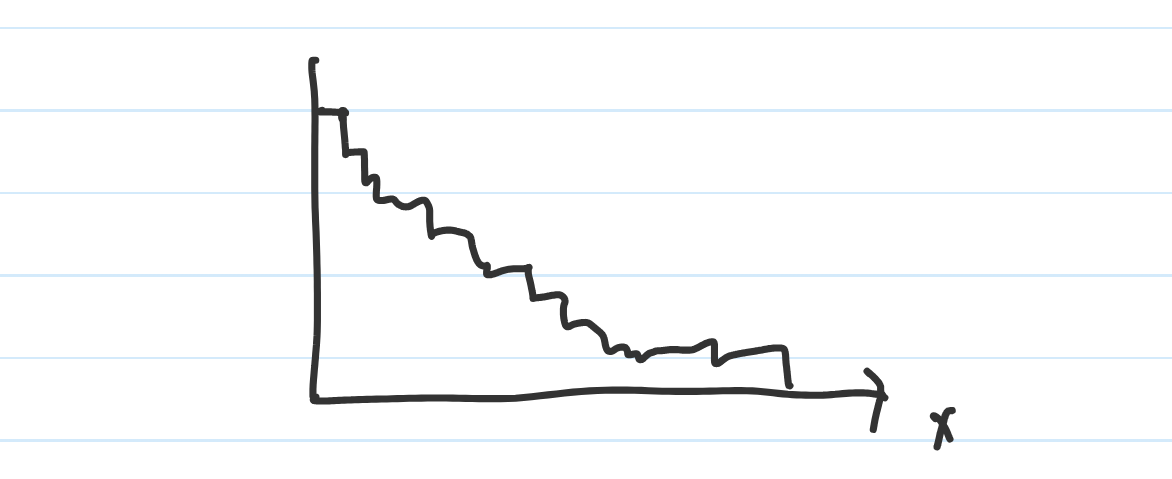
\includegraphics[width=0.4\linewidth]{Images/lec11-histogram.png}

                    Say the resolution has:

                    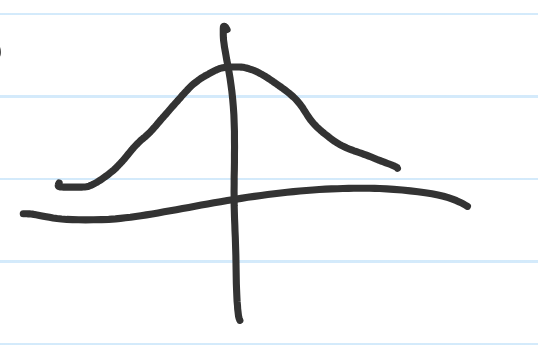
\includegraphics[width=0.4\linewidth]{Images/lec11-resolution.png}

                    so what you see is actually a convolution of the true distribution with the resolution function.

                    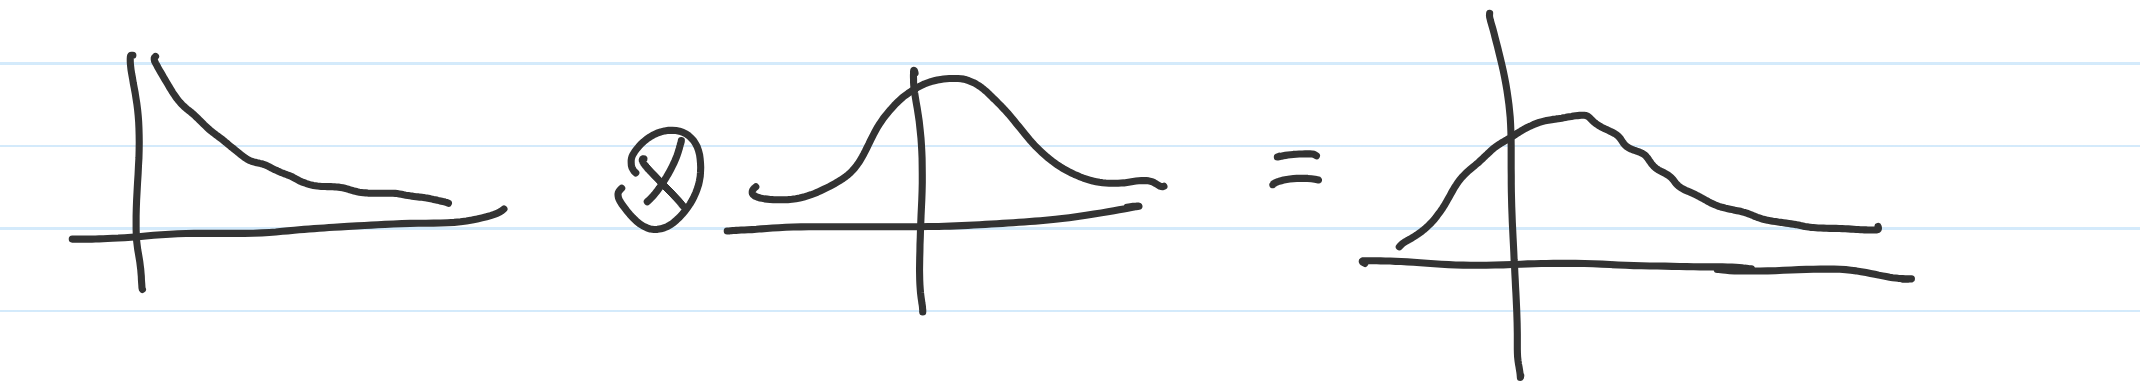
\includegraphics[width=0.4\linewidth]{Images/lec11-convolution.png}

                    So the fit should actually be an exponential $\circledast$ Gaussian in this case.

                    \[
                        \chi^2 = \sum_i \frac{(n_i - f_i(\theta))^2}{\sigma_i^2}
                    \]

                    Suppose we expect Poisson statistics:

                    \[
                        \sigma_i^2 = n_i
                    \]

                    Then the data are weighted by $n_i$:

                    \[
                        \text{Neyman } \chi^2 \equiv \sum_i \frac{(n_i - f_i(\theta))^2}{n_i}
                    \]

                    which is a modified least squares form.

                    Alternatively, it is sensible to say that the expected entries are given by our model:

                    \[
                        \Rightarrow \text{ use } f_i(\vec{\theta}) \text{ as the mean.}
                    \]

                    Therefore:

                    \[
                        \text{Pearson } \chi^2 \equiv \sum_i \frac{(n_i - f_i(\theta))^2}{f_i(\theta)}
                    \]

                    For Neyman $\chi^2$, if a bin is empty ($n_i = 0$) then it diverges.
                    Both Neyman and Pearson forms are biased in opposite ways.
                    One could use Neyman and Pearson together, but is it worth the effort?
          \end{enumerate}
\end{itemize}
